% ****** Start of file apssamp.tex ******
%
%   This file is part of the APS files in the REVTeX 4.1 distribution.
%   Version 4.1r of REVTeX, August 2010
%
%   Copyright (c) 2009, 2010 The American Physical Society.
%
%   See the REVTeX 4 README file for restrictions and more information.
%
% TeX'ing this file requires that you have AMS-LaTeX 2.0 installed
% as well as the rest of the prerequisites for REVTeX 4.1
%
% See the REVTeX 4 README file
% It also requires running BibTeX. The commands are as follows:
%
%  1)  latex apssamp.tex
%  2)  bibtex apssamp
%  3)  latex apssamp.tex
%  4)  latex apssamp.tex
%
\documentclass[%
 reprint,
superscriptaddress,
%groupedaddress,
%unsortedaddress,
%runinaddress,
%frontmatterverbose,
%preprint,
showpacs,
% preprintnumbers,
%nofootinbib,
%nobibnotes,
%bibnotes,
 amsmath,amssymb,
 aps,
% prx,
%pra,
 prb,
%rmp,
%prstab,
%prstper,
%floatfix,
longbibliography,
]{revtex4-1}

\usepackage{graphicx}% Include figure files
\usepackage{dcolumn}% Align table columns on decimal point
\usepackage{bm}% bold math
\usepackage{xcolor}
\usepackage{hyperref}% add hypertext capabilities
\usepackage{afterpage}
\usepackage{bbold}
%\usepackage[mathlines]{lineno}% Enable numbering of text and display math
%\linenumbers\relax % Commence numbering lines

\newcommand{\infint}[1]{\int\limits_{-\infty}^{\infty}{#1}}

\begin{document}

\title{Notes on numerical stabilization in determinant quantum Monte Carlo}% Force line breaks with \\

\author{Carsten Bauer}
\affiliation{Institute for Theoretical Physics, University of Cologne, 50937 Cologne, Germany}

\date{\today}% It is always \today, today,
             %  but any date may be explicitly specified

\begin{abstract}
In these notes we will empirically compare different matrix decompositions for use in numerical stabilization in many-body quantum Monte Carlo simulation, in particular when calculating equal time Green's functions. We will both benchmark their speed and accuracy. We will further show that special care has to be taken when calculating time-displaced Green's functions and will review a well-known but somewhat hard to find method for stabilizing the necessary inversion in this case. We will focus on and use the Julia programming language for all calculations. An implementation of all discussed methods is available in the open-source software library \href{http://github.com/crstnbr/StableDQMC.jl}{StableDQMC.jl}.
\end{abstract}


\maketitle

%\tableofcontents

\section{\label{sec:why}The issue}

\subsubsection{Determinant quantum Monte Carlo in a nutshell}

For the description of the DQMC algorithm, we consider a quantum field theory that can be split into a purely bosonic part $S_B$ and a part $S_F$, which comprises fermion kinetics $T$ and boson-fermion interactions $V$. An example is the famous Hubbard model after decoupling the on-site
interaction $U n_{i, \uparrow} n_{i, \downarrow}$ by means of a Hubbard-Stratonovich or Hirsch transformation in either the spin or charge channel \cite{Hirsch1983}. As per usual, the central quantity of interest is the partition function
%
\begin{equation}
\mathcal{Z} = \int D\left( \psi, \psi^\dagger, \phi \right) e^{-S_B - S_F} \,.
\end{equation}
%
The basic idea is to switch from the $d$ dimensional quantum theory to a $D = d + 1$ dimensional classical theory as in the path integral framework. The first step is to discretize and Trotter decompose the imaginary time $\tau$,
%
\begin{align}
	\mathcal{Z} &= \int D\phi \ e^{-S_B} \mathrm{Tr}{\left[\exp{\left( -\Delta\tau \sum_{l=1}^M \psi^\dagger \left[T + V_\phi\right] \psi \right)}\right]} \label{eq:discretizedpi} \,.
\end{align}
%
The exponential is then separated and the appearing commutator ignored which results in a systematic error of the order $\mathcal{O}\left(\Delta\tau^2\right)$,
\begin{align}
	e^{A + B} &\approx e^A e^B \quad \nonumber\\
	e^{-\Delta\tau (T + V)} &\approx e^{- \frac{\Delta\tau}{2}T} e^{-\Delta\tau V} e^{- \frac{\Delta\tau}{2}T} + \mathcal{O}\left(\Delta\tau^3\right), \nonumber\\
	\mathcal{Z} &= \int D\phi \ e^{-S_B} \mathrm{Tr}{\left[ \prod_{l=1}^{m} B_l \right]} + \mathcal{O}\left(\Delta\tau^2\right). \label{eq:Ztr}
\end{align}
%
Note that the potential part $e^{-\Delta\tau \psi^\dagger V_\phi \psi}$ in the time-slice propagators $B_l = e^{- \frac{\Delta\tau}{2}\psi^\dagger T \psi} e^{-\Delta\tau \psi^\dagger V_\phi \psi} e^{- \frac{\Delta\tau}{2}\psi^\dagger T \psi}$ depends on the boson $\phi$ due to the present fermion-boson coupling. Rewriting the trace in \eqref{eq:Ztr} as a determinant, an identity which can be proven \textcolor{red}{CITE}, yields the fundamental form
%
\begin{align}
	\mathcal{Z} &= \int D\phi \ e^{-S_B} \det{G_\phi^{-1}} + \mathcal{O}\left(\Delta\tau^2\right),
\end{align}
%
where
\begin{align}
	G = \left( \mathbb{1} + B_M B_{M-1} \cdots B_1 \right)^{-1} \label{etgf}
\end{align}
is the equal-time Green's function.

Only under specific circumstances, such as the presence of a symmetry, can the integral kernel be safely be interpreted as a probability weight, as $G_\phi$ and its determinant are generally complex valued (\textit{sign problem}).

\subsubsection{Numerical instabilities}

\begin{figure}[h]
	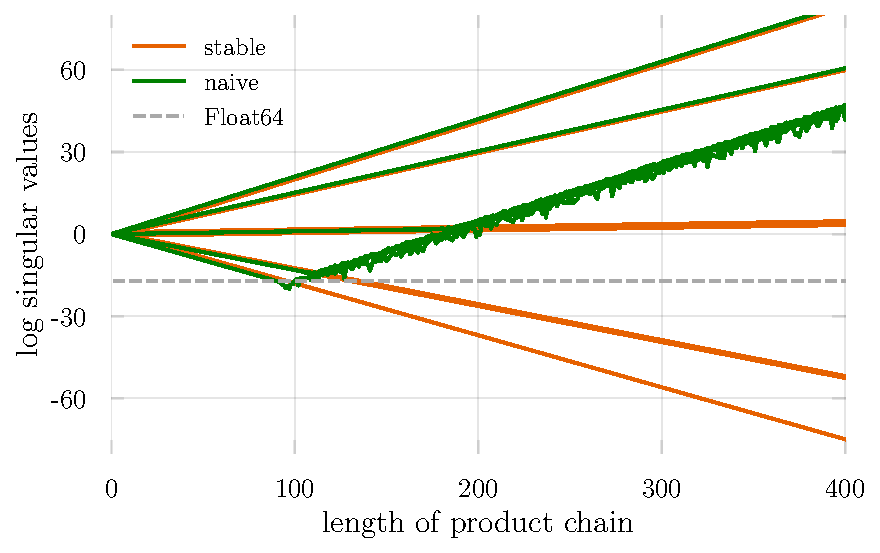
\includegraphics[width=0.5\textwidth]{../../examples/naive_vs_stable.pdf}
	\caption{Simple model \label{fig:naive_vs_stable}}
\end{figure}

\begin{figure}[h]
	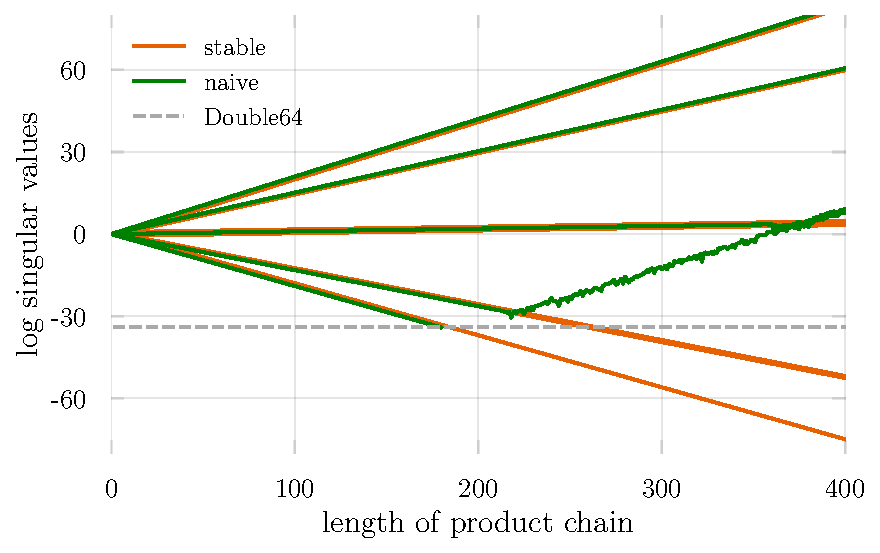
\includegraphics[width=0.5\textwidth]{../../examples/naive_vs_stable_db64.pdf}
	\caption{Simple model \label{fig:naive_vs_stable_db64}}
\end{figure}

\section{\label{sec:decompositions}Matrix decompositions for the rescue}

\subsubsection{SVD}

\subsubsection{QR}

\subsubsection{Gram-Schmidt}


\section{Benchmarks}

\subsection{Accuracy}

\begin{figure}[h]
	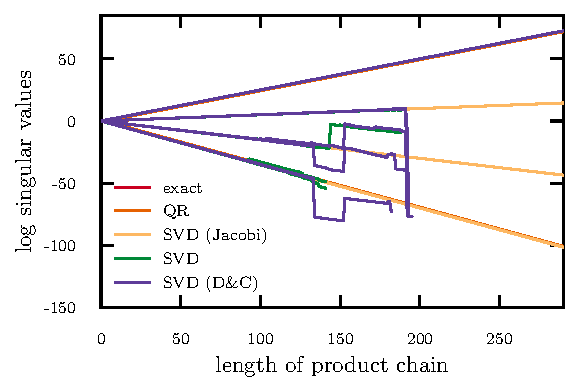
\includegraphics[width=0.5\textwidth]{../../examples/decomp_comparison.pdf}
	\caption{Spin-fermion model at $\beta = 40$ \label{fig:decomp_comparison}}
\end{figure}

\begin{figure}[h]
	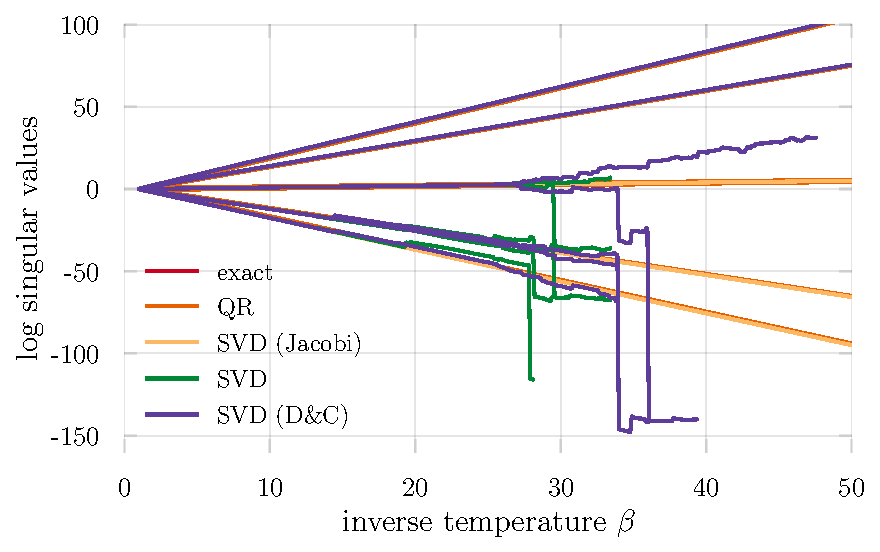
\includegraphics[width=0.5\textwidth]{../../examples/decomp_comparison_simple.pdf}
	\caption{Simple model system \label{fig:decomp_comparison_simple}}
\end{figure}

%\begin{figure}[h]
%	\includegraphics[width=0.5\textwidth]{../../examples/svd_comparison.pdf}
%	\caption{$\beta = 40$ \label{fig:svd_comparison}}
%\end{figure}



\subsection{Efficiency}



%\section{The time-displaced Green's function}










%\afterpage{\clearpage}
\clearpage
\bibliography{references}
%\clearpage
%\appendix


\end{document}
%
% ****** End of file apssamp.tex ******
